\documentclass[conference]{IEEEtran}
\IEEEoverridecommandlockouts
\usepackage{cite}
\usepackage{amsmath,amssymb,amsfonts}
\usepackage{graphicx}
\usepackage{booktabs}
\usepackage{array}
\usepackage{url}
\usepackage{tikz}
\usetikzlibrary{positioning,arrows.meta}
\usepackage[hidelinks]{hyperref}
\graphicspath{{figures/}}

\begin{document}

\title{Deep Learning-Based Plant Health Classification Using a Self-Collected Rooftop Garden Image Dataset}

\author{\IEEEauthorblockN{Abubakar Siddiq Sazzad}
\IEEEauthorblockA{Department of Computer Science and Engineering\\
International University of Scholars\\
Email: siddiqsazzad001@gmail.com}}

\maketitle

\begin{abstract}
Plant image classification is an important computer-vision task with applications in crop monitoring, home gardening, and agricultural decision support. This paper presents a small-scale experimental study on visible plant-health condition classification using a self-collected image dataset obtained from a rooftop garden. Instead of relying on a large public plant-disease benchmark, the study constructs a local dataset of 64 photographs and organizes them into five visually defined categories: Healthy, Yellowing/Discoloration, Leaf Spot/Browning, Dry/Severe Damage, and Insect/Physical Damage. A MobileNetV2 convolutional neural network pretrained on ImageNet is used as a transfer-learning feature extractor, followed by global average pooling, dropout, and a five-class softmax classifier. The dataset is divided into training, validation, and test subsets containing 43, 8, and 13 images, respectively. Training uses image augmentation and 15 epochs of optimization with Adam. The baseline experiment obtains approximately 48.8\% training accuracy, 50.0\% validation accuracy, and 46.15\% test accuracy. On the test set, the macro-averaged F1-score is 0.13 and the weighted F1-score is 0.29. The confusion matrix shows that all 13 test images were assigned to the Healthy class, including the six correctly classified healthy examples. These results demonstrate the feasibility of implementing an end-to-end self-collected image-classification pipeline, but they also show that the present dataset is too small and imbalanced to support strong generalization claims. The reported experiment is therefore treated as a baseline, with dataset expansion, improved class balance, and controlled preprocessing experiments identified as the main directions for future work.
\end{abstract}

\begin{IEEEkeywords}
deep learning, image classification, convolutional neural network, MobileNetV2, transfer learning, plant health, rooftop garden, self-collected dataset
\end{IEEEkeywords}

\section{Introduction}
Image classification has become a central task in computer vision because a trained model can learn visual patterns from labeled images and assign previously unseen images to predefined categories. Convolutional neural networks (CNNs) are particularly effective for visual recognition because they learn hierarchical representations of image structure. Large-scale datasets such as ImageNet have supported the development of general-purpose visual representations and pretrained models \cite{deng2009imagenet}.

Plant monitoring is one application area where image classification can provide useful assistance. Leaves may show visible changes such as yellowing, browning, drying, spots, holes, and other forms of physical damage. Earlier research demonstrated that deep learning can classify plant images under controlled conditions. Mohanty, Hughes, and Salath\'e used a large public dataset to classify crop species and disease categories, but also reported a substantial performance reduction when models were evaluated on images collected under different conditions \cite{mohanty2016}. This observation is important for small real-world datasets because illumination, background, camera distance, plant variety, leaf orientation, and environmental conditions can vary considerably.

This work studies a different setting: a small dataset collected directly from a rooftop garden. The goal is not to diagnose a specific biological disease from a photograph. Instead, the task is defined as classification of five visually observable plant-health conditions. This distinction is important because the labels are based on visible appearance rather than laboratory testing or expert-confirmed pathogen diagnosis.

A major practical challenge is the limited number of available images. Deep CNNs can require substantial data to learn robust task-specific representations, while augmentation can increase the variety of training examples when only a small dataset is available \cite{shorten2019}. Transfer learning provides another practical strategy: representations learned from a large source dataset can be reused for a smaller target problem. Yosinski et al. showed that transferred features can provide useful general representations, although transferability depends on the relationship between source and target tasks \cite{yosinski2014}.

The research question addressed in this baseline study is: \emph{Can a transfer-learning CNN provide a useful baseline for classifying visible plant-health conditions in a small, self-collected rooftop-garden image dataset?}

The main contributions are:
\begin{itemize}
\item creation and documentation of a 64-image self-collected rooftop-garden dataset;
\item definition of five visually observable plant-health condition categories;
\item implementation of a MobileNetV2 transfer-learning classification pipeline;
\item evaluation using accuracy, precision, recall, F1-score, and a confusion matrix; and
\item analysis of the effects of the small and imbalanced dataset on the baseline results.
\end{itemize}

\section{Related Work}
\subsection{Plant Image Classification}
Deep learning has been widely investigated for plant image analysis. Mohanty et al. trained deep neural networks on more than 54,000 plant images covering multiple crops and disease categories and demonstrated the potential of image-based disease recognition \cite{mohanty2016}. Their study also showed that performance can fall considerably when a model is tested on imagery collected under conditions different from the training data. The present study therefore emphasizes images collected from the actual target environment rather than relying only on a public benchmark.

The sample paper supplied for this project also uses deep learning for plant image classification. Its general research structure motivates the organization of the present paper, but the present study uses a different self-collected dataset and a different baseline configuration. The categories in this work describe visible conditions and are not claims of confirmed biological diseases.

\subsection{Transfer Learning}
Training a deep model from random initialization can be difficult when the target dataset is small. Transfer learning starts from parameters learned on a large source dataset and adapts them to a new task. Yosinski et al. studied the generality and specificity of deep features and found that lower-level features can transfer across tasks while higher-level features become more task-specific \cite{yosinski2014}. This motivates using a pretrained convolutional base and training a smaller task-specific classification head.

\subsection{MobileNetV2}
MobileNetV2 was introduced by Sandler et al. using inverted residual blocks and linear bottlenecks \cite{sandler2018}. The architecture was designed to balance visual representation quality with computational efficiency. This makes it a practical baseline for a small image-classification project and a possible future candidate for resource-constrained deployment.

The TensorFlow/Keras implementation provides ImageNet-pretrained MobileNetV2 weights and model-specific preprocessing functionality \cite{tensorflow_mobilenetv2}. The current baseline reports the preprocessing that was actually used in the project notebook, as described in Section IV.

\subsection{Data Augmentation and Evaluation}
Image augmentation can increase training variation through transformations such as rotation, shifting, zooming, and flipping. A survey by Shorten and Khoshgoftaar discusses augmentation as a practical approach for limited-data deep-learning settings \cite{shorten2019}. Because the present dataset is small, moderate augmentation is applied only to the training split.

For imbalanced multi-class problems, reporting multiple evaluation measures is useful. Sokolova and Lapalme provide a systematic analysis of classification performance measures and discuss the role of macro- and class-based evaluation \cite{sokolova2009}. Accordingly, this study reports accuracy together with class-wise precision, recall, F1-score, macro averages, weighted averages, and a confusion matrix.

\section{Dataset and Data Collection}
\subsection{Self-Collected Rooftop Dataset}
The dataset was collected from a rooftop garden using photographs of leaves and plant parts. The images contain natural variation in lighting, background, leaf orientation, camera distance, and visible damage. The dataset was organized manually into five visually defined classes.

A key design decision was to avoid assigning a biological disease name without sufficient evidence. For example, ``Yellowing/Discoloration'' refers to an observed color change, while ``Insect/Physical Damage'' refers to visible holes or physical damage. The labels should therefore be interpreted as visual-condition categories rather than definitive diagnoses.

\begin{table}[!t]
\centering
\caption{Composition of the Self-Collected Dataset}
\label{tab:dataset}
\begin{tabular}{lrr}
\toprule
\textbf{Class} & \textbf{Images} & \textbf{Percentage}\\
\midrule
Healthy & 31 & 48.44\%\\
Yellowing/Discoloration & 10 & 15.63\%\\
Leaf Spot/Browning & 13 & 20.31\%\\
Dry/Severe Damage & 6 & 9.38\%\\
Insect/Physical Damage & 4 & 6.25\%\\
\midrule
\textbf{Total} & \textbf{64} & \textbf{100.00\%}\\
\bottomrule
\end{tabular}
\end{table}

The largest class contains 31 images while the smallest contains four, giving a 7.75:1 ratio between the largest and smallest classes.

\begin{figure}[!t]
\centering
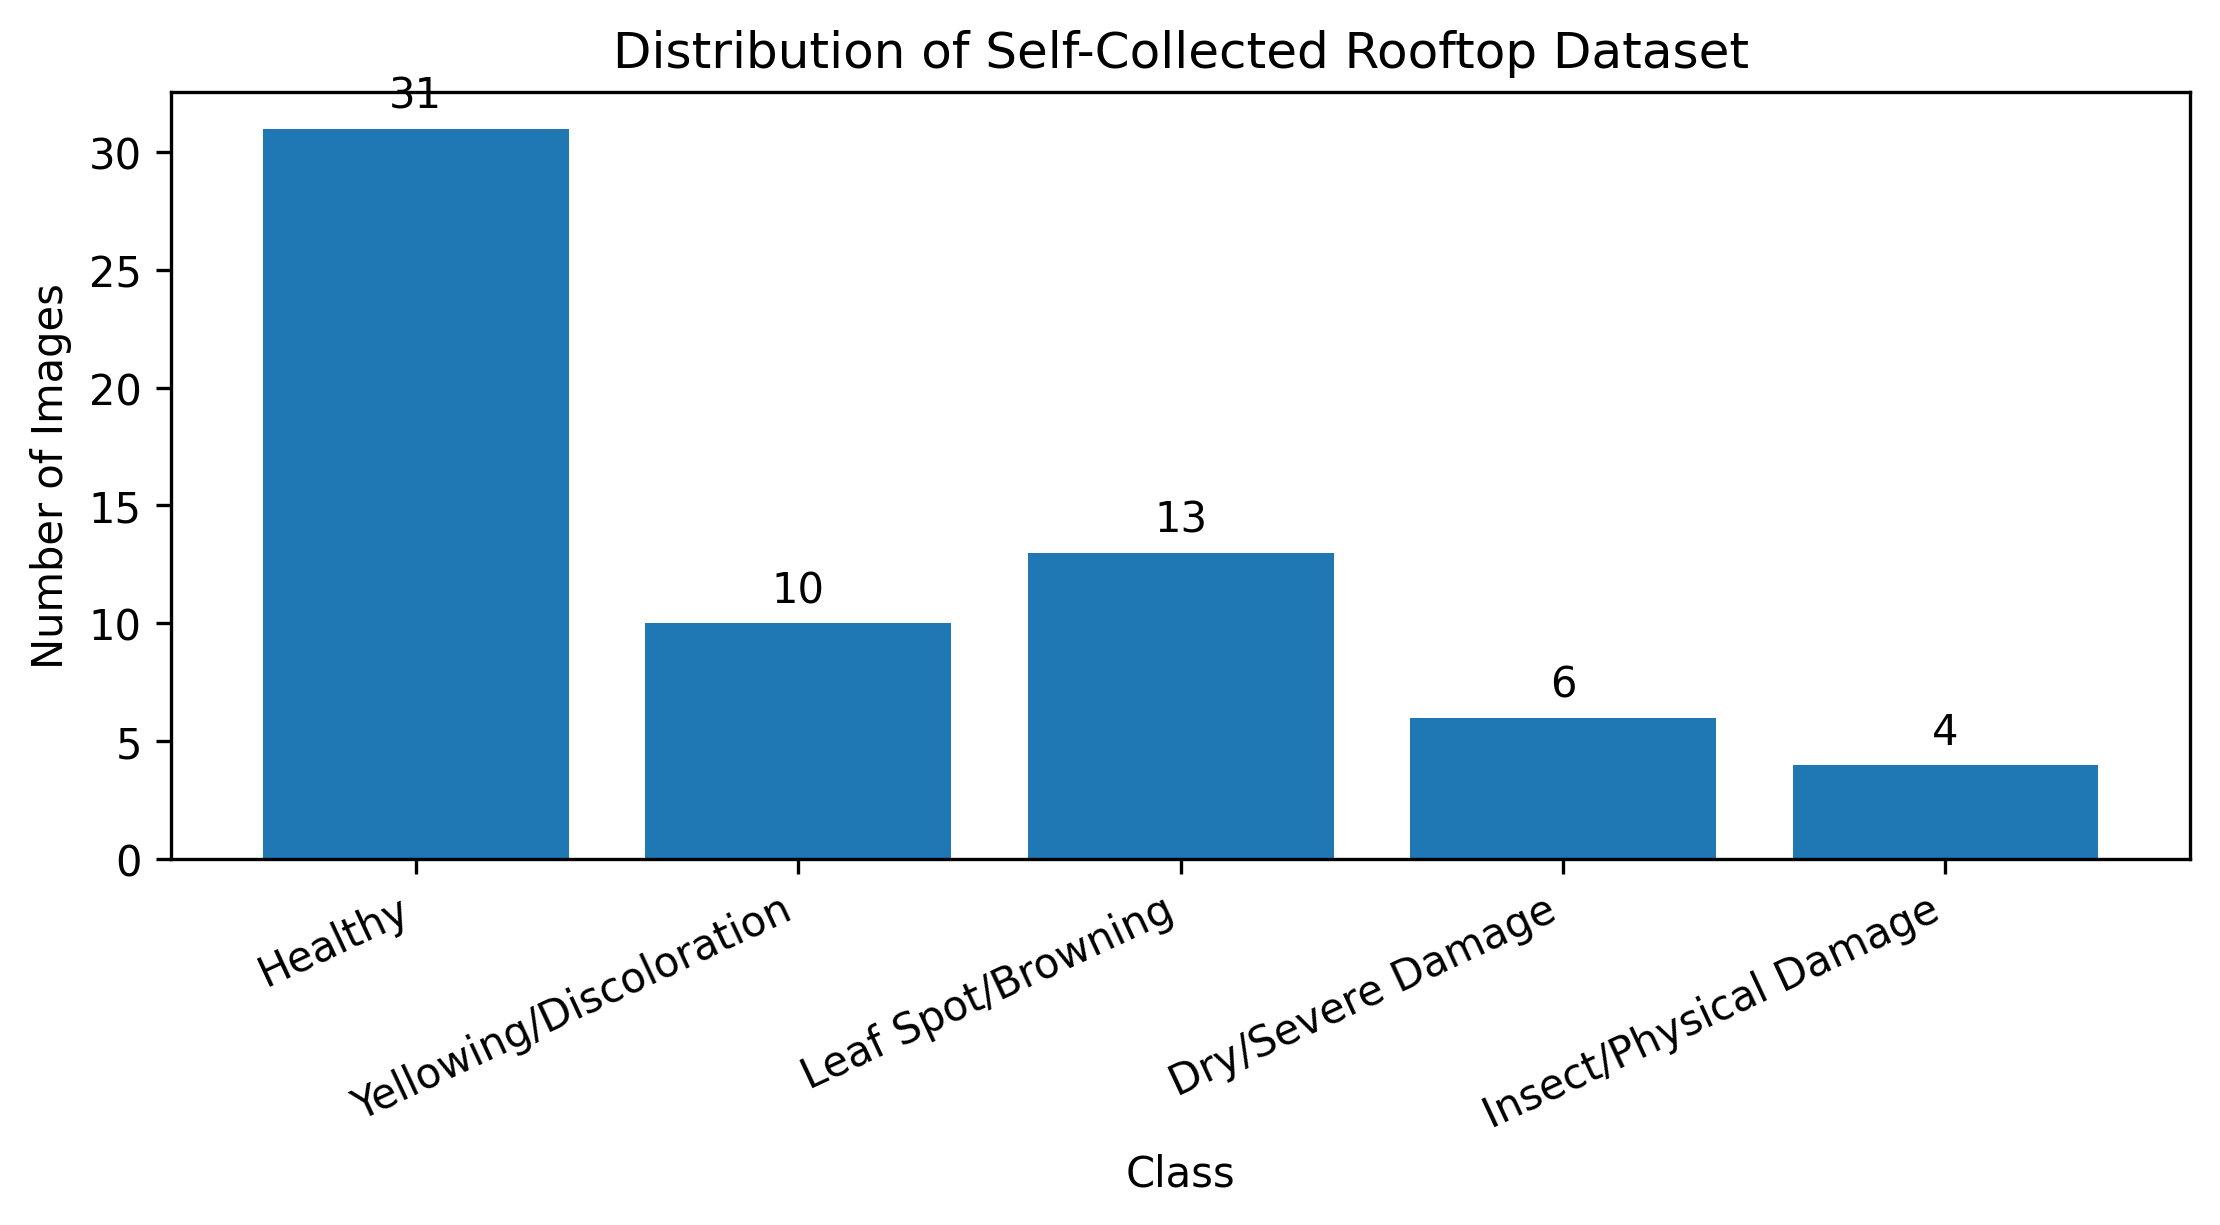
\includegraphics[width=\columnwidth]{dataset_distribution.png}
\caption{Distribution of the 64 images across the five visible-condition classes.}
\label{fig:distribution}
\end{figure}

\subsection{Representative Samples}
Figure~\ref{fig:samples} shows representative images from all five categories. These examples illustrate the visual nature of the classification task.

\begin{figure*}[!t]
\centering
\begin{minipage}{0.18\textwidth}\centering
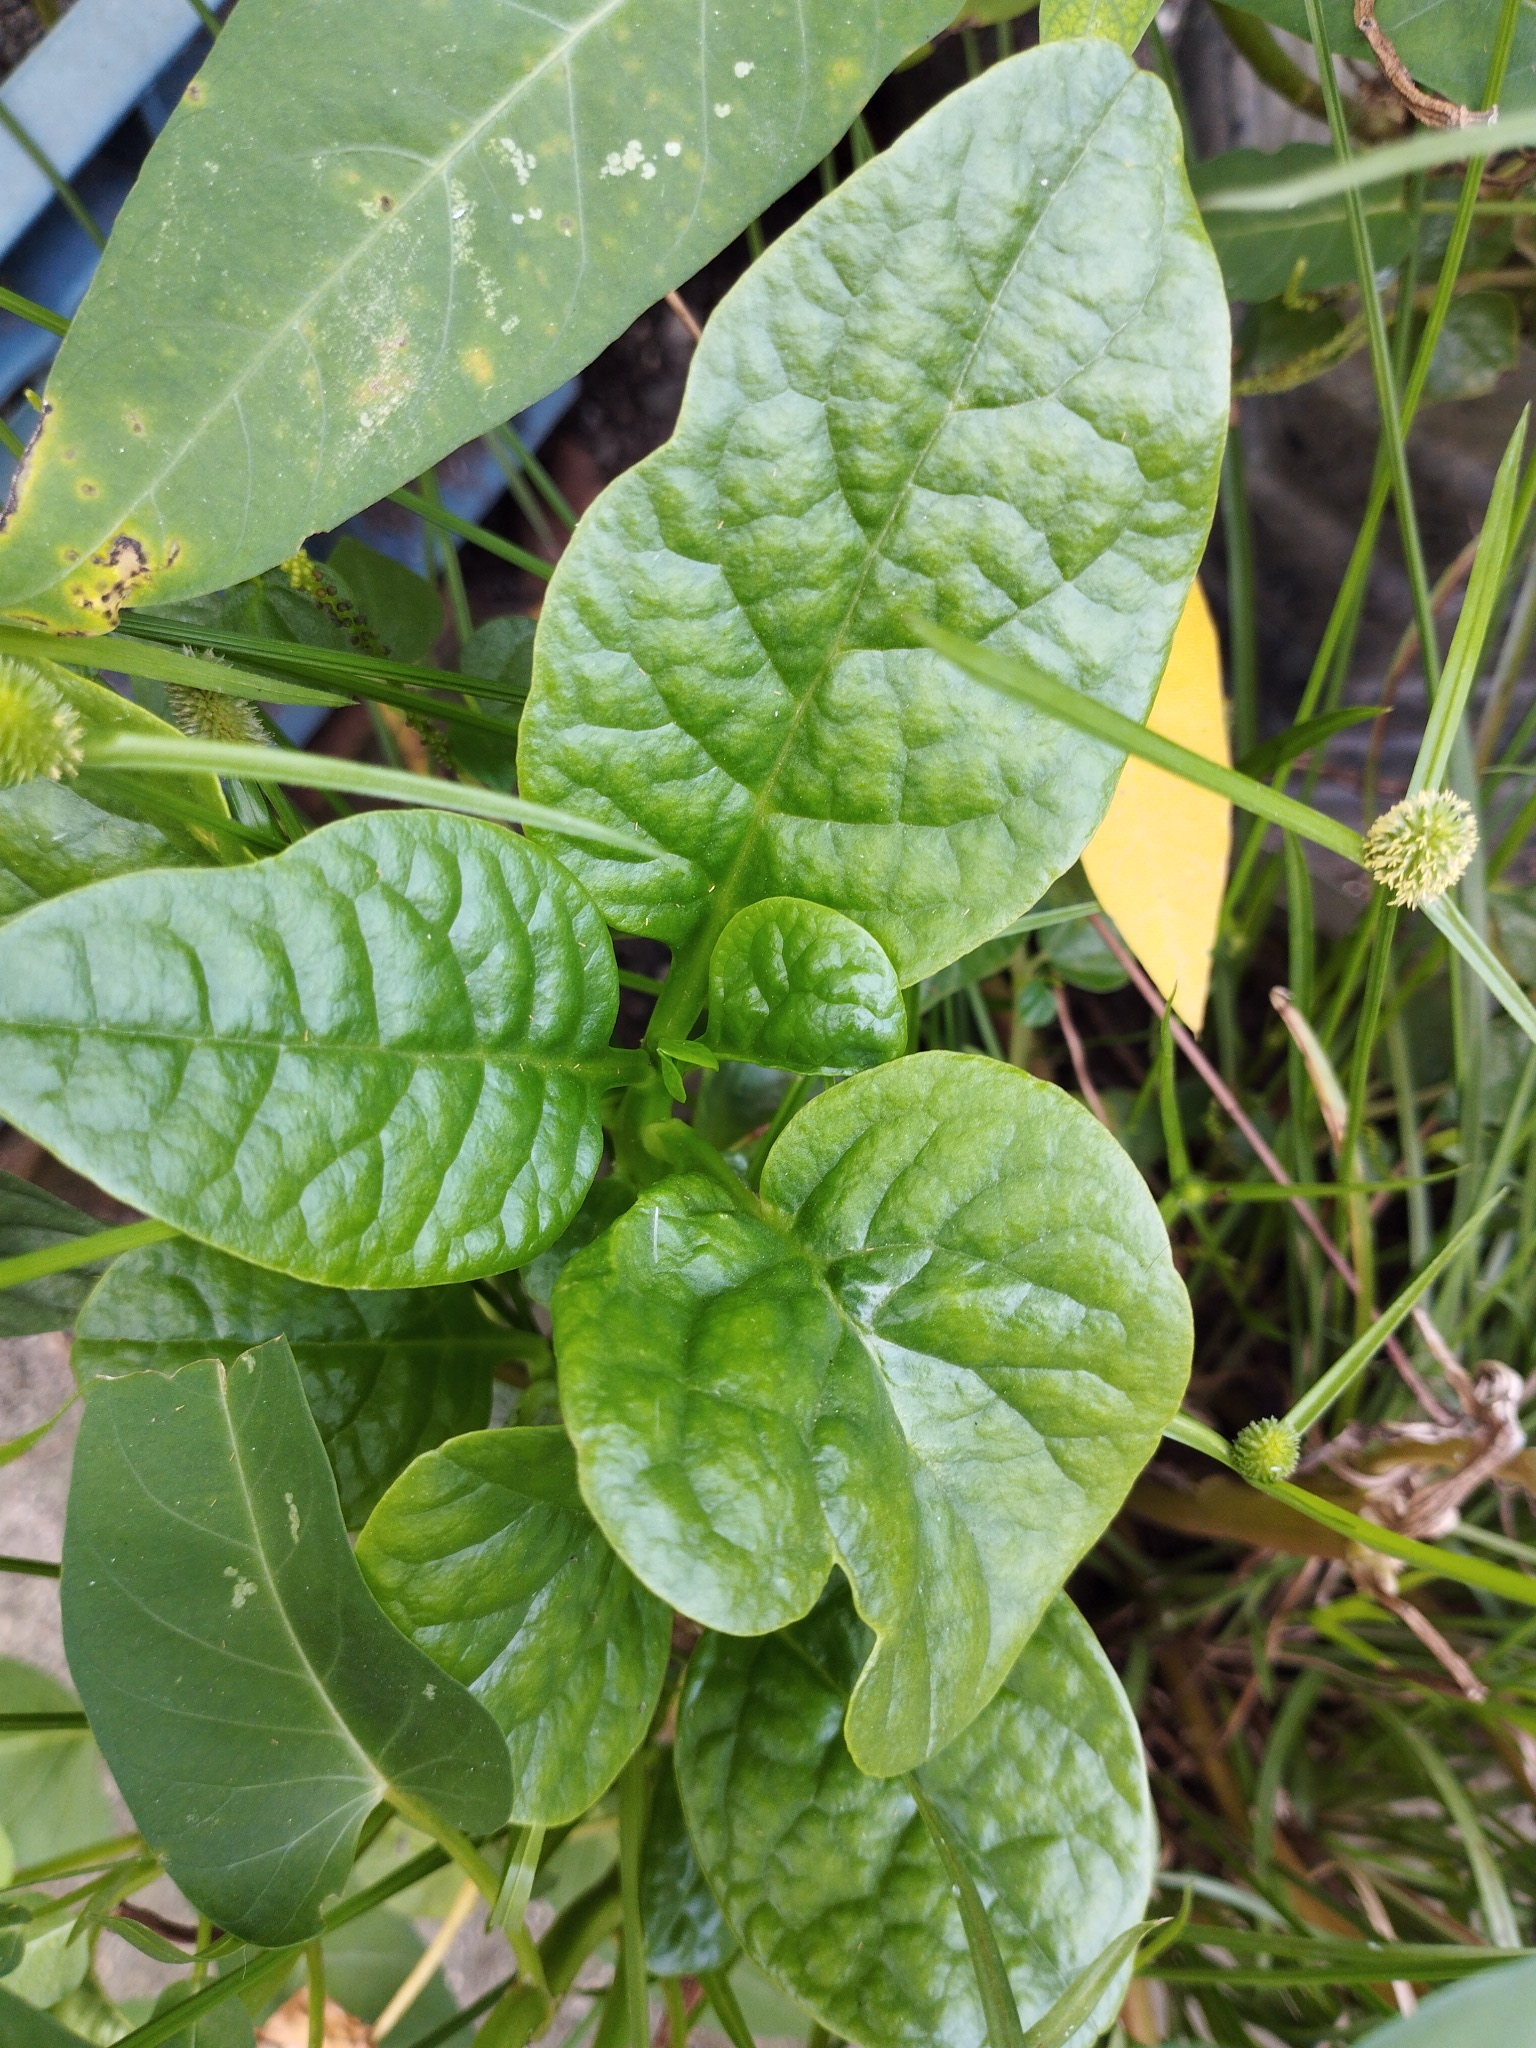
\includegraphics[width=\linewidth,height=4.0cm,keepaspectratio]{Healthy.jpg}\\
\scriptsize (a) Healthy\end{minipage}\hfill
\begin{minipage}{0.18\textwidth}\centering
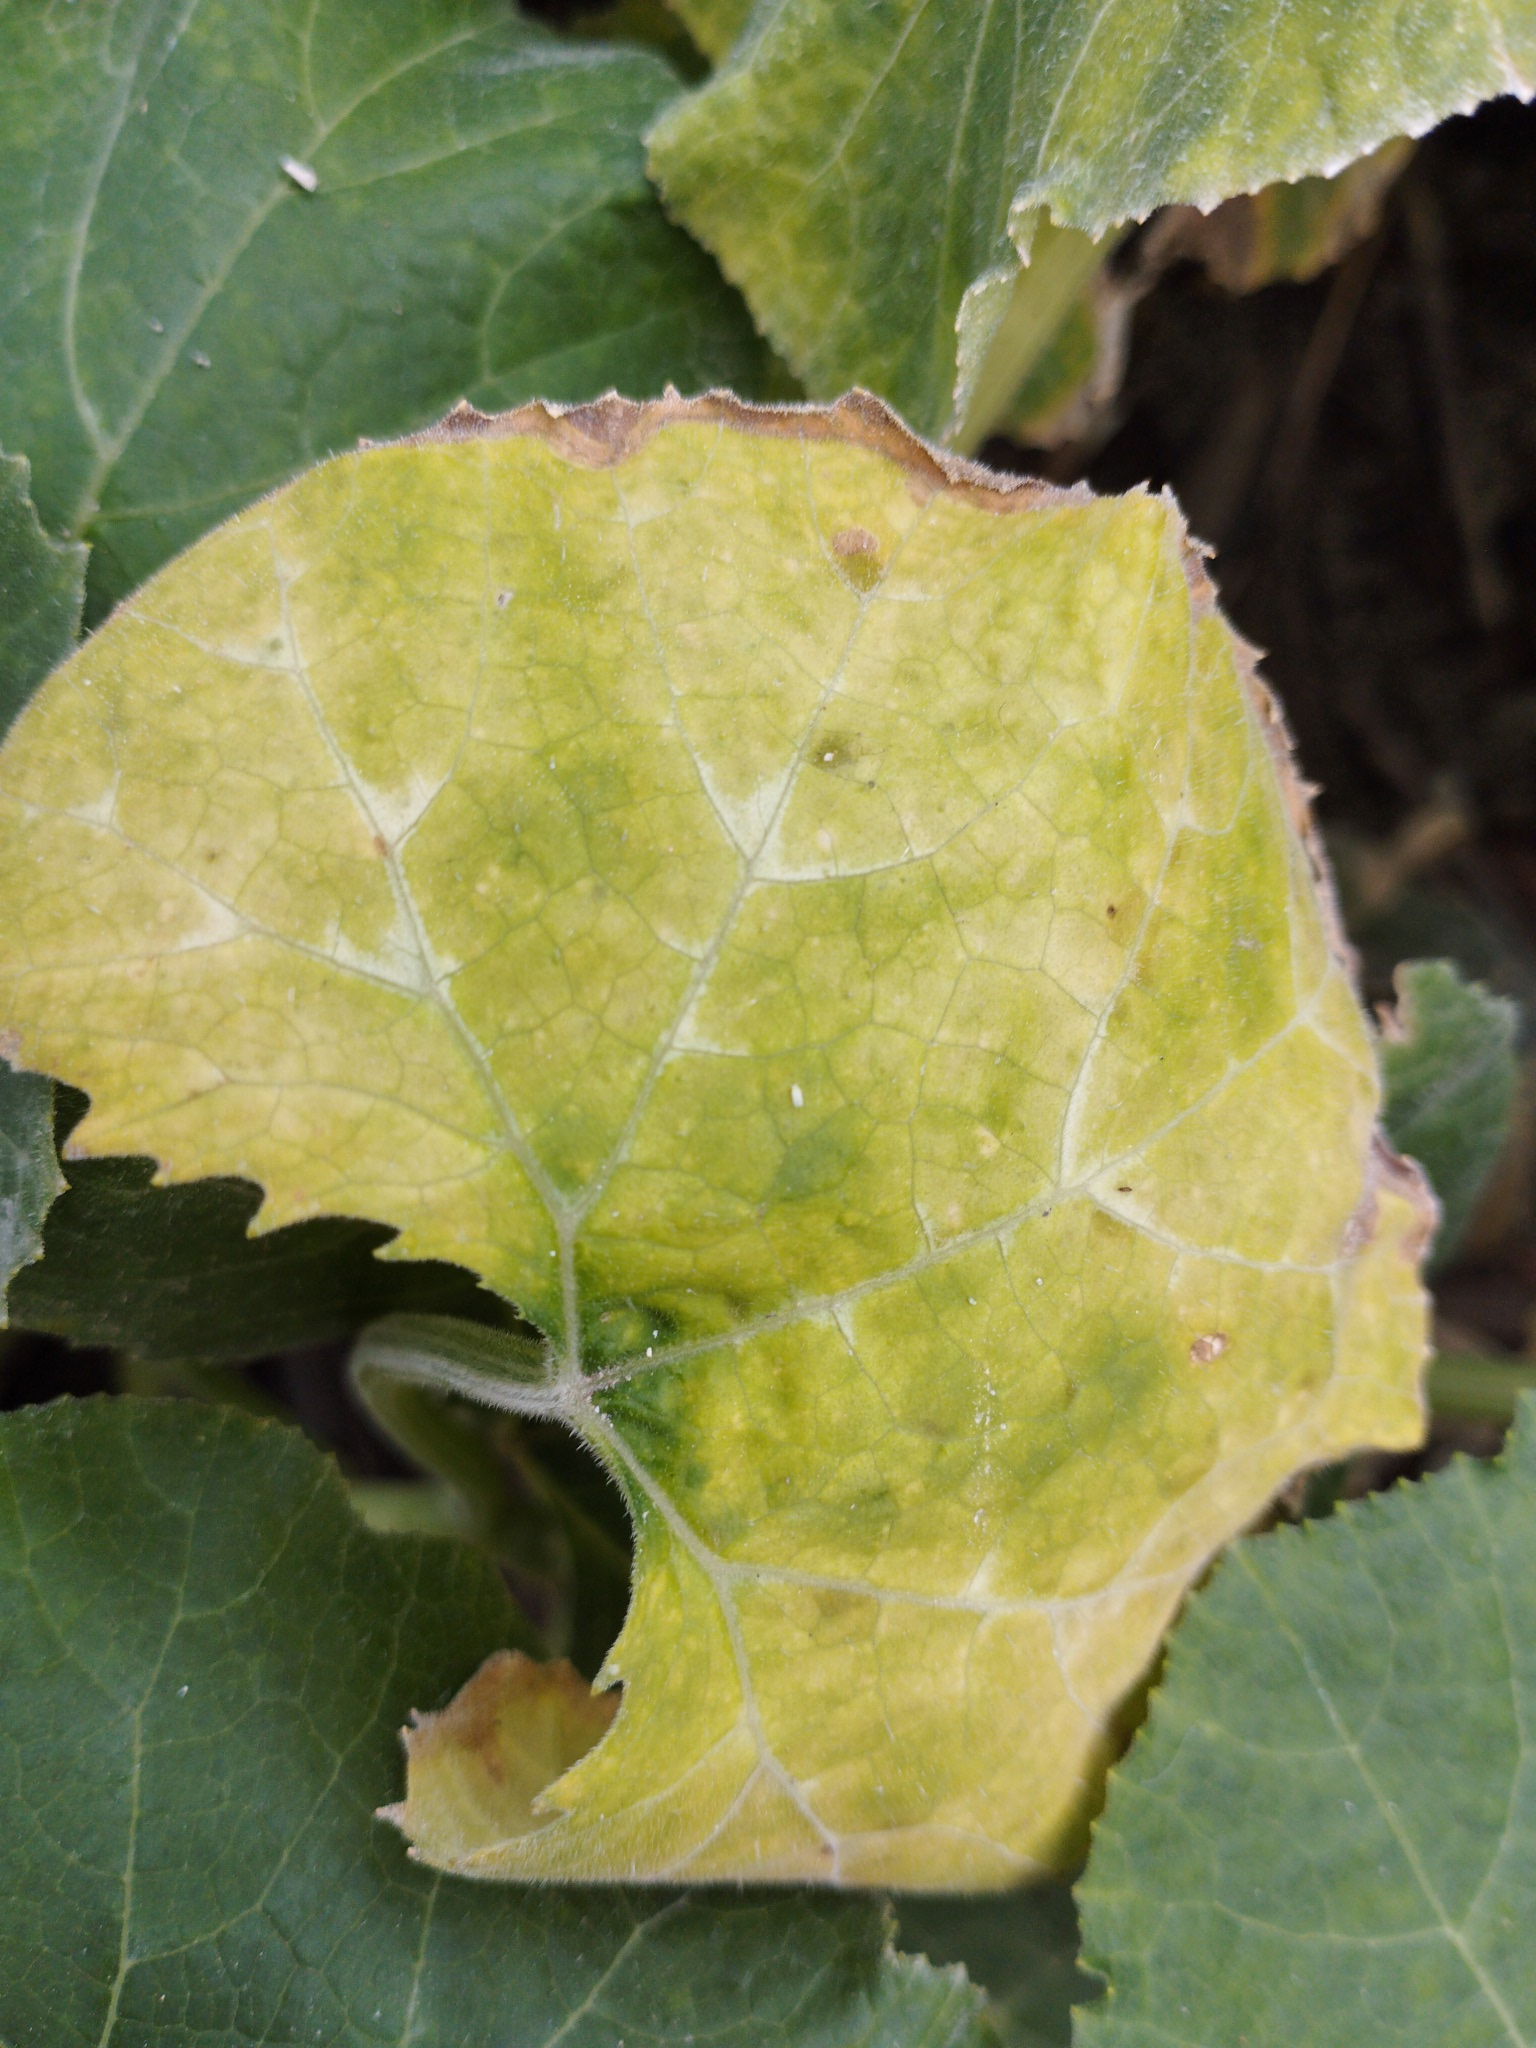
\includegraphics[width=\linewidth,height=4.0cm,keepaspectratio]{Yellowing_Discoloration.jpg}\\
\scriptsize (b) Yellowing/Discoloration\end{minipage}\hfill
\begin{minipage}{0.18\textwidth}\centering
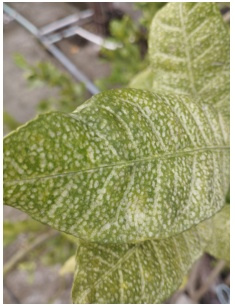
\includegraphics[width=\linewidth,height=4.0cm,keepaspectratio]{Leaf_Spot_Browning.jpg}\\
\scriptsize (c) Leaf Spot/Browning\end{minipage}\hfill
\begin{minipage}{0.18\textwidth}\centering
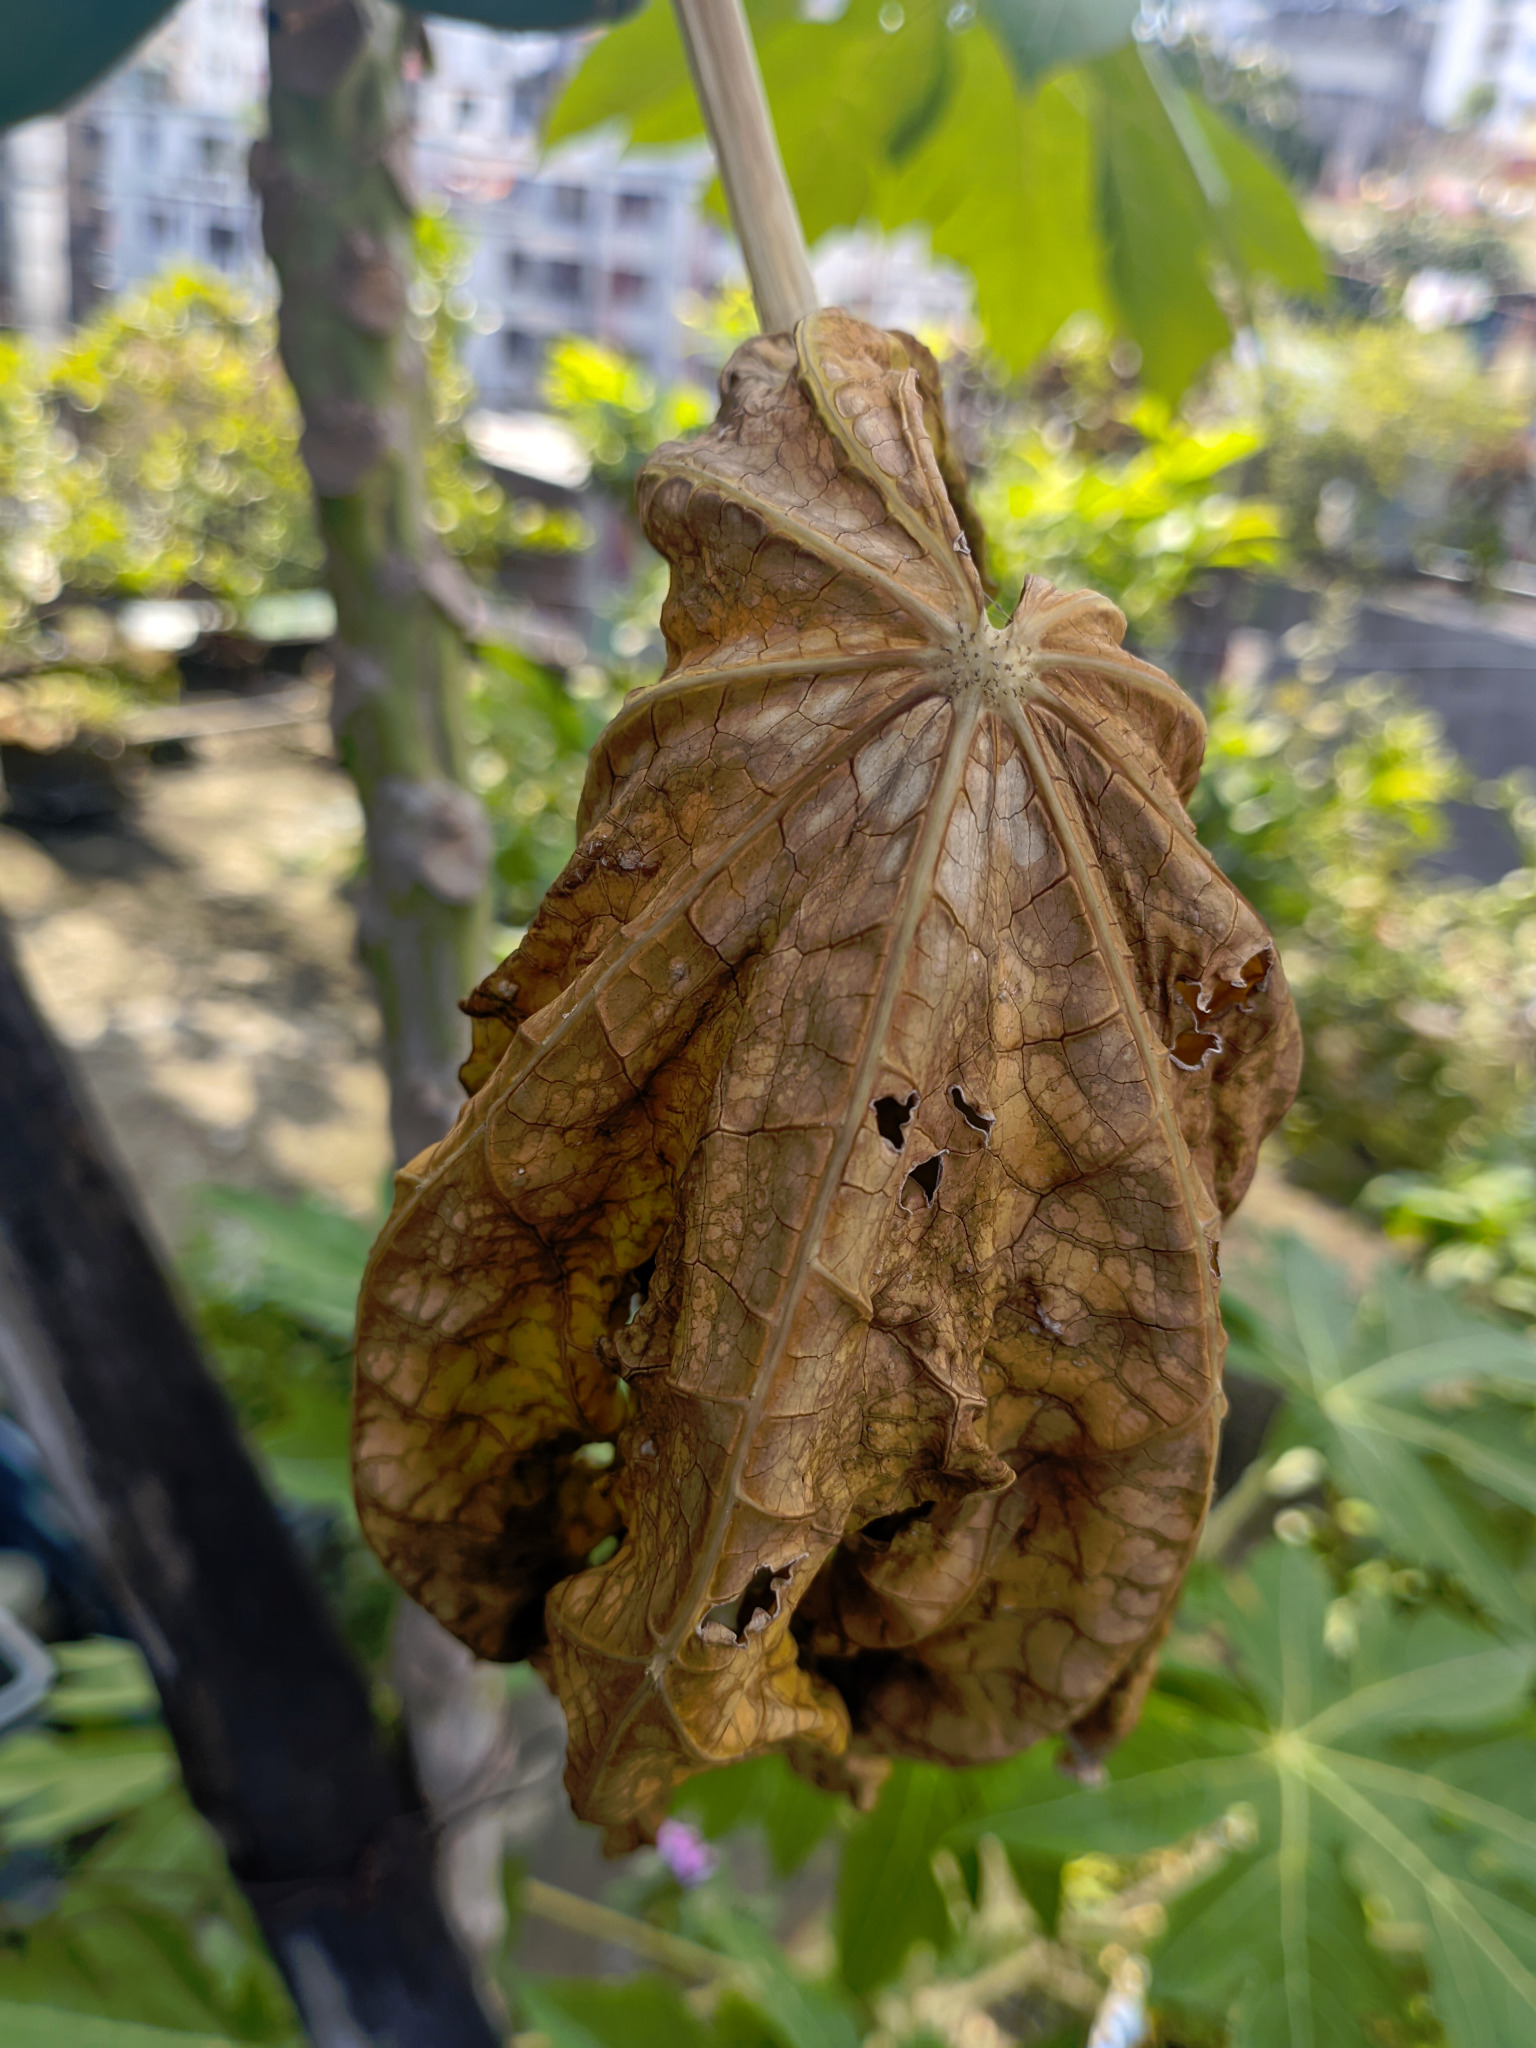
\includegraphics[width=\linewidth,height=4.0cm,keepaspectratio]{Dry_Severe_Damage.jpg}\\
\scriptsize (d) Dry/Severe Damage\end{minipage}\hfill
\begin{minipage}{0.18\textwidth}\centering
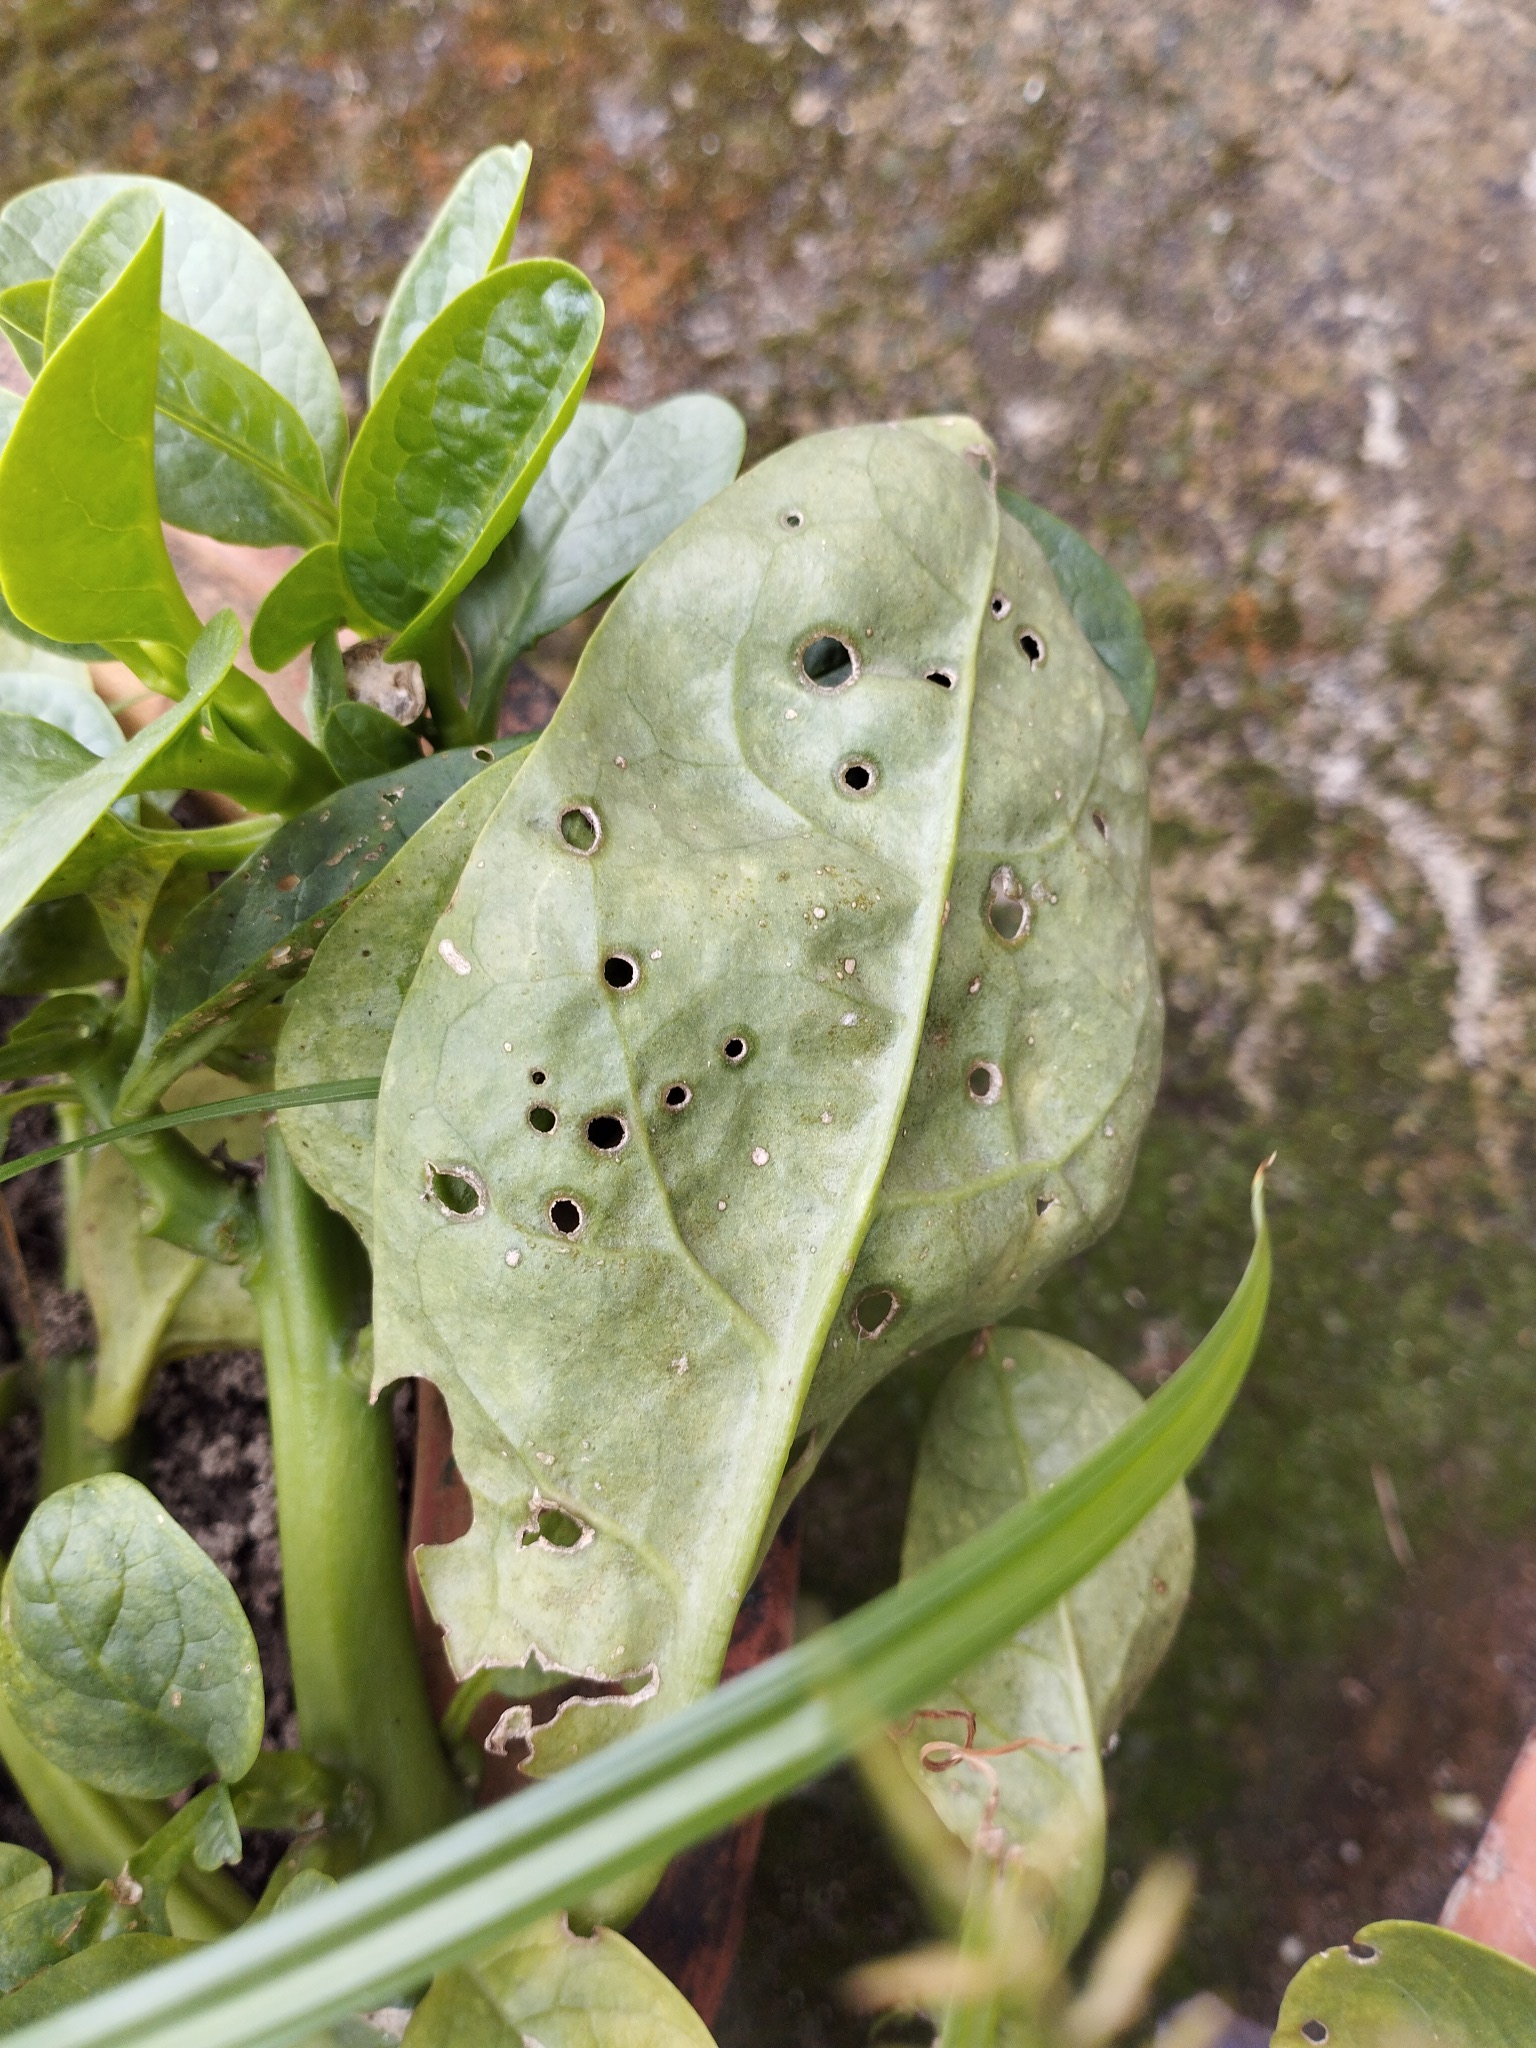
\includegraphics[width=\linewidth,height=4.0cm,keepaspectratio]{Insect_Physical_Damage.jpg}\\
\scriptsize (e) Insect/Physical Damage\end{minipage}
\caption{Representative images from the five visible-condition categories in the self-collected rooftop dataset.}
\label{fig:samples}
\end{figure*}

\subsection{Dataset Splitting}
The notebook uses random seed 42 and approximately a 70/15/15 split for each class. The implementation ensures at least one validation and one test image for every category. The resulting split contains 43 training images, 8 validation images, and 13 test images.

\begin{table}[!t]
\centering
\caption{Class Distribution Across Dataset Splits}
\label{tab:split}
\resizebox{\columnwidth}{!}{\begin{tabular}{lrrr}
\toprule
\textbf{Class} & \textbf{Train} & \textbf{Validation} & \textbf{Test}\\
\midrule
Healthy & 21 & 4 & 6\\
Yellowing/Discoloration & 7 & 1 & 2\\
Leaf Spot/Browning & 9 & 1 & 3\\
Dry/Severe Damage & 4 & 1 & 1\\
Insect/Physical Damage & 2 & 1 & 1\\
\midrule
\textbf{Total} & \textbf{43} & \textbf{8} & \textbf{13}\\
\bottomrule
\end{tabular}}
\end{table}

The split is performed before augmentation. The notebook also checks filename overlap among the three subsets and reports zero overlap. This prevents the same original filename from appearing in multiple subsets.

\section{Methodology}
\subsection{Overall Workflow}
The complete pipeline consists of image collection, visible-condition labeling, dataset splitting, preprocessing, training augmentation, MobileNetV2 transfer learning, classification, and evaluation. Figure~\ref{fig:workflow} summarizes the process.

\begin{figure}[!t]
\centering
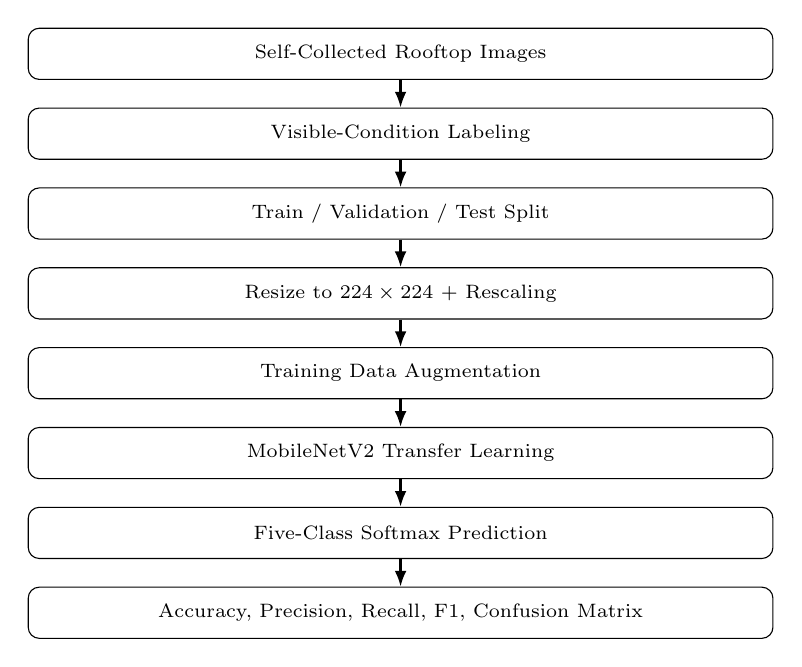
\begin{tikzpicture}[node distance=3.5mm,
box/.style={draw,rounded corners,align=center,minimum width=0.78\columnwidth,minimum height=6.5mm,font=\scriptsize},
arrow/.style={-{Latex[length=2mm]},thick}]
\node[box] (a) {Self-Collected Rooftop Images};
\node[box,below=of a] (b) {Visible-Condition Labeling};
\node[box,below=of b] (c) {Train / Validation / Test Split};
\node[box,below=of c] (d) {Resize to $224\times224$ + Rescaling};
\node[box,below=of d] (e) {Training Data Augmentation};
\node[box,below=of e] (f) {MobileNetV2 Transfer Learning};
\node[box,below=of f] (g) {Five-Class Softmax Prediction};
\node[box,below=of g] (h) {Accuracy, Precision, Recall, F1, Confusion Matrix};
\draw[arrow](a)--(b);\draw[arrow](b)--(c);\draw[arrow](c)--(d);\draw[arrow](d)--(e);\draw[arrow](e)--(f);\draw[arrow](f)--(g);\draw[arrow](g)--(h);
\end{tikzpicture}
\caption{Overall workflow of the rooftop plant-health classification experiment.}
\label{fig:workflow}
\end{figure}

\subsection{Image Preprocessing}
All images are resized to $224\times224$ pixels. The project notebook uses Keras \texttt{ImageDataGenerator} with a rescaling factor of $1/255$, so the baseline inputs are approximately in the range $[0,1]$.

The official TensorFlow documentation states that MobileNetV2-specific preprocessing scales pixel values to $[-1,1]$ \cite{tensorflow_mobilenetv2}. The current experiment was executed using $1/255$ rescaling rather than the model-specific \texttt{preprocess\_input} function. This implementation detail is reported explicitly for reproducibility. It is also an important improvement target for the next experiment.

\subsection{Data Augmentation}
The training generator applies rotation up to 20 degrees, width and height shifts up to 10\%, zoom up to 15\%, horizontal flipping, and $1/255$ rescaling. Validation and test images receive only the rescaling operation. Applying augmentation only to the training set avoids modifying the evaluation samples.

\subsection{MobileNetV2 Model}
The baseline model uses MobileNetV2 with ImageNet-pretrained weights and \texttt{include\_top=False}. The convolutional base is frozen. Global average pooling converts the convolutional features to a compact vector, followed by dropout with rate 0.3 and a dense five-unit softmax classifier.

\begin{equation}
\mathbf{x}_{224\times224\times3}\rightarrow\mathrm{MobileNetV2}\rightarrow\mathrm{GAP}\rightarrow\mathrm{Dropout}(0.3)\rightarrow\mathrm{Dense}(5)\rightarrow\mathrm{Softmax}.
\end{equation}

\begin{figure}[!t]
\centering
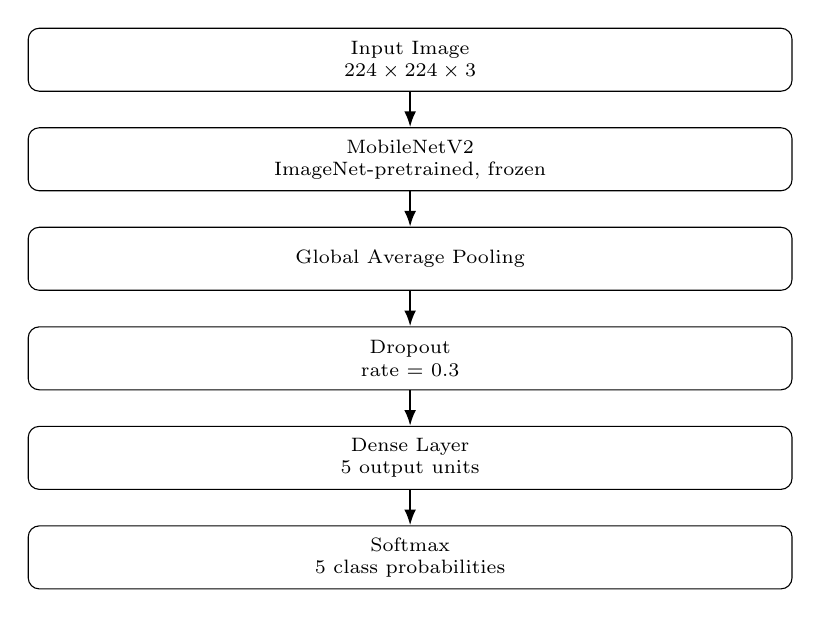
\begin{tikzpicture}[node distance=4.5mm,
box/.style={draw,rounded corners,align=center,minimum width=0.80\columnwidth,minimum height=8mm,font=\scriptsize},
arrow/.style={-{Latex[length=2mm]},thick}]
\node[box](a){Input Image\\$224\times224\times3$};
\node[box,below=of a](b){MobileNetV2\\ImageNet-pretrained, frozen};
\node[box,below=of b](c){Global Average Pooling};
\node[box,below=of c](d){Dropout\\rate = 0.3};
\node[box,below=of d](e){Dense Layer\\5 output units};
\node[box,below=of e](f){Softmax\\5 class probabilities};
\draw[arrow](a)--(b);\draw[arrow](b)--(c);\draw[arrow](c)--(d);\draw[arrow](d)--(e);\draw[arrow](e)--(f);
\end{tikzpicture}
\caption{Baseline MobileNetV2 transfer-learning architecture.}
\label{fig:architecture}
\end{figure}

\subsection{Training Configuration}
The model is trained for 15 epochs with batch size 8, Adam optimizer, learning rate 0.0001, and categorical cross-entropy loss.

\begin{table}[!t]
\centering
\caption{Baseline Training Configuration}
\label{tab:training}
\begin{tabular}{ll}
\toprule
\textbf{Parameter} & \textbf{Value}\\
\midrule
Architecture & MobileNetV2\\
Pretrained weights & ImageNet\\
Input size & $224\times224\times3$\\
Base model & Frozen\\
Classes & 5\\
Batch size & 8\\
Epochs & 15\\
Optimizer & Adam\\
Learning rate & 0.0001\\
Dropout & 0.30\\
Loss & Categorical cross-entropy\\
Random seed & 42\\
\bottomrule
\end{tabular}
\end{table}

\subsection{Evaluation Metrics}
Accuracy is the proportion of correct predictions:
\begin{equation}
Accuracy=\frac{\text{correct predictions}}{\text{total predictions}}.
\end{equation}
For class $i$, precision, recall, and F1-score are
\begin{equation}
Precision_i=\frac{TP_i}{TP_i+FP_i},\qquad
Recall_i=\frac{TP_i}{TP_i+FN_i},
\end{equation}
\begin{equation}
F1_i=2\frac{Precision_i\times Recall_i}{Precision_i+Recall_i}.
\end{equation}
Macro averaging gives equal importance to all classes, which is useful when class sizes differ substantially \cite{sokolova2009}.

\section{Experimental Results}
\subsection{Training and Validation Accuracy}
Figure~\ref{fig:accuracy} shows the 15-epoch accuracy history. Training accuracy fluctuates from approximately 16\% at the beginning to approximately 48.8\% at the final epoch. Validation accuracy reaches 50\% and remains at approximately that level during the later epochs.

\begin{figure}[!t]
\centering
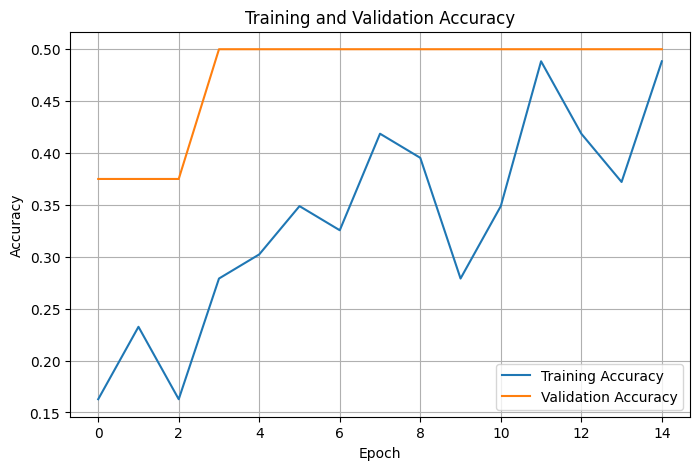
\includegraphics[width=\columnwidth]{Training_and_Validation_Accuracy.png}
\caption{Training and validation accuracy over 15 epochs.}
\label{fig:accuracy}
\end{figure}

Because only 43 images are used for training and eight for validation, individual samples have a large effect on the curves. The validation accuracy should therefore not be interpreted as a stable estimate of generalization.

\subsection{Training and Validation Loss}
Figure~\ref{fig:loss} presents the loss history. Training loss decreases overall but fluctuates, while validation loss decreases initially and later rises. This pattern is consistent with limited generalization in the small-data baseline, although the eight-image validation set makes the estimate highly uncertain.

\begin{figure}[!t]
\centering
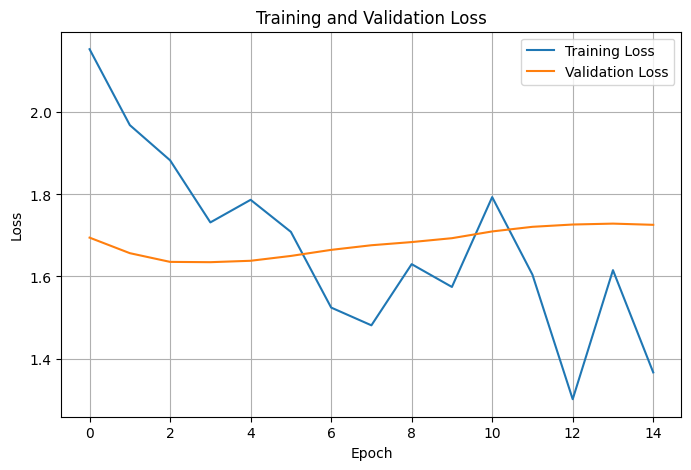
\includegraphics[width=\columnwidth]{Training_and_Validation_Loss.png}
\caption{Training and validation loss over 15 epochs.}
\label{fig:loss}
\end{figure}

\subsection{Test Performance}
The test set contains 13 images. The measured test loss is 1.7034 and test accuracy is 46.15\%. Since six of the thirteen test images are Healthy, a model that predicts Healthy for every test image would also obtain $6/13=46.15\%$ accuracy. The confusion matrix confirms that the baseline effectively behaves this way.

\begin{table}[!t]
\centering
\caption{Baseline Experimental Results}
\label{tab:results}
\begin{tabular}{lr}
\toprule
\textbf{Metric} & \textbf{Value}\\
\midrule
Final training accuracy & $\approx48.8\%$\\
Final validation accuracy & $50.0\%$\\
Test loss & 1.7034\\
Test accuracy & $46.15\%$\\
Macro precision & 0.09\\
Macro recall & 0.20\\
Macro F1 & 0.13\\
Weighted precision & 0.21\\
Weighted recall & 0.46\\
Weighted F1 & 0.29\\
\bottomrule
\end{tabular}
\end{table}

\subsection{Class-Wise Classification Report}
Table~\ref{tab:report} gives the test-set classification report. Healthy is the only class with non-zero recall. The other classes have zero recall because none of their test examples was predicted correctly.

\begin{table}[!t]
\centering
\caption{Class-Wise Test Classification Report}
\label{tab:report}
\resizebox{\columnwidth}{!}{\begin{tabular}{lrrrr}
\toprule
\textbf{Class} & \textbf{Prec.} & \textbf{Recall} & \textbf{F1} & \textbf{Support}\\
\midrule
Dry/Severe Damage & 0.00 & 0.00 & 0.00 & 1\\
Healthy & 0.46 & 1.00 & 0.63 & 6\\
Insect/Physical Damage & 0.00 & 0.00 & 0.00 & 1\\
Leaf Spot/Browning & 0.00 & 0.00 & 0.00 & 3\\
Yellowing/Discoloration & 0.00 & 0.00 & 0.00 & 2\\
\midrule
Macro average & 0.09 & 0.20 & 0.13 & 13\\
Weighted average & 0.21 & 0.46 & 0.29 & 13\\
\bottomrule
\end{tabular}}
\end{table}

\subsection{Confusion Matrix}
Figure~\ref{fig:cm} shows six correct Healthy predictions and thirteen total predictions in the Healthy column. Specifically, one Dry/Severe Damage image, one Insect/Physical Damage image, three Leaf Spot/Browning images, and two Yellowing/Discoloration images were also predicted as Healthy.

\begin{figure}[!t]
\centering
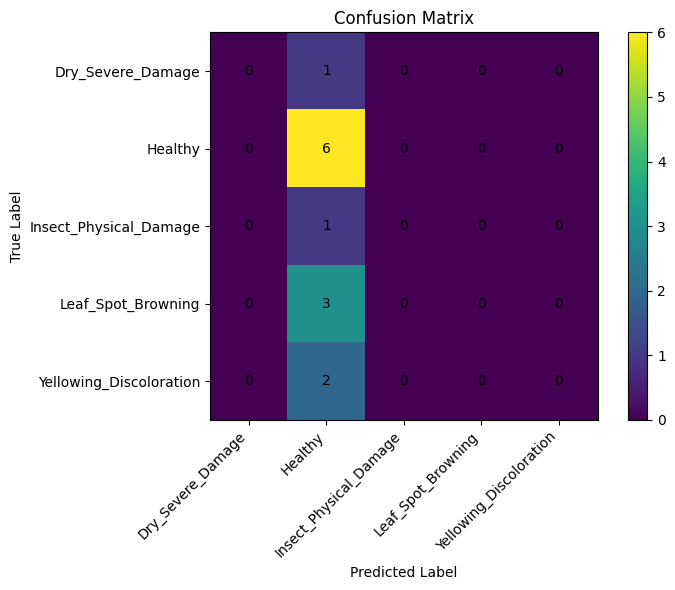
\includegraphics[width=\columnwidth]{Confusion_Matrix.png}
\caption{Confusion matrix for the 13-image test set.}
\label{fig:cm}
\end{figure}

\section{Discussion}
\subsection{Interpretation of the Baseline}
The experiment successfully implements an end-to-end workflow from real image collection to CNN training and quantitative evaluation. However, the results should be treated as a preliminary baseline rather than evidence that the system can reliably classify plant health in general.

The most important result is the mismatch between overall accuracy and class-wise performance. The 46.15\% test accuracy is not evidence of balanced five-class recognition because it is exactly the majority-class baseline for this test set. The macro F1-score of 0.13 provides a clearer summary of performance across all categories.

\subsection{Class Imbalance}
Class imbalance is a major limitation. The complete dataset contains 31 Healthy images but only four Insect/Physical Damage images. After splitting, the minority class has only two training images, one validation image, and one test image. Dry/Severe Damage also has only four training images.

This scarcity makes it difficult for the model to learn the visual variability of minority conditions. It also makes test metrics unstable: for a class with only one test image, one correct prediction changes recall from 0 to 1. The difference between macro F1 (0.13) and weighted F1 (0.29) further illustrates the effect of class distribution.

\subsection{Dataset Size and Augmentation}
Only 64 original images are available, with 43 used for training. Augmentation increases the number of transformed training samples but does not create new independent physical observations. Consequently, additional real images are the most important improvement. Future collection should include multiple plants, leaves, viewpoints, lighting conditions, and severity levels for each class.

\subsection{Preprocessing Consideration}
The baseline notebook uses $1/255$ rescaling. TensorFlow documents MobileNetV2-specific preprocessing that maps pixel values to $[-1,1]$ \cite{tensorflow_mobilenetv2}. Therefore, the current experiment does not use the standard MobileNetV2 preprocessing function. This does not change the reported results because the paper documents the actual implementation, but a future controlled experiment should use the official preprocessing and compare it with the current baseline.

\subsection{External Validity and Label Scope}
The dataset comes from one rooftop garden and therefore does not represent all crops, climates, gardens, camera devices, or environmental conditions. The model should not be presented as a general agricultural diagnostic system. Furthermore, visible yellowing, spots, drying, or holes can have multiple causes. Without expert or laboratory confirmation, the categories in this paper are visual-condition labels rather than confirmed biological diagnoses.

\section{Limitations and Future Work}
The main limitations are the small sample size, strong class imbalance, very small validation and test sets, single-garden collection environment, single baseline architecture, and non-standard MobileNetV2 input scaling used in the executed notebook.

Future work should first expand the real dataset, especially the minority classes. A stronger dataset should include more independent images per class, different lighting conditions, different camera distances, multiple plants, and multiple stages of visible damage. The second step should be a controlled rerun using the official MobileNetV2 preprocessing function. The third step should compare additional pretrained architectures while keeping the split and evaluation protocol fixed. Once enough data are collected, repeated stratified evaluation or cross-validation can provide more reliable estimates.

An additional future direction is an ``Unknown/Uncertain'' category or confidence threshold. A practical system should not be forced to assign every image to one of five classes when an image is ambiguous or outside the training distribution. This extension would require new data and dedicated evaluation.

\section{Conclusion}
This paper presented a deep-learning image-classification pipeline for visible plant-health conditions using a self-collected rooftop-garden dataset. The dataset contains 64 photographs organized into five categories: Healthy, Yellowing/Discoloration, Leaf Spot/Browning, Dry/Severe Damage, and Insect/Physical Damage. A MobileNetV2 model with ImageNet-pretrained weights was used as a frozen feature extractor followed by global average pooling, dropout, and a five-class softmax classifier.

The baseline used 43 training images, 8 validation images, and 13 test images. After 15 epochs, the model achieved approximately 48.8\% training accuracy, 50.0\% validation accuracy, and 46.15\% test accuracy. The macro F1-score was 0.13. The confusion matrix showed that all test samples were predicted as Healthy, so the reported test accuracy is equivalent to the majority-class baseline for this test set.

The primary value of the study is the creation of a reproducible pipeline based on real rooftop-garden images and the identification of the data limitations that prevent strong generalization. Future experiments should increase the number and diversity of real images, improve class balance, use official MobileNetV2 preprocessing, and evaluate the resulting models on a larger and more representative test set.

\bibliographystyle{IEEEtran}
\bibliography{references}
\end{document}
